\documentclass[11pt]{article}
\usepackage[margin=1in]{geometry}
\usepackage{graphicx}
\usepackage{booktabs}
\usepackage{amsmath}
\usepackage{amssymb}
\usepackage[hidelinks]{hyperref}
\usepackage{microtype}
\emergencystretch=3em
\graphicspath{{../figures/}}

\title{When does fusion help? Multiplicative cross-modal fusion for
voice-clone scam detection, and the limits of off-the-shelf detectors}
\author{Author Name \\ \texttt{dulam@nvidia.com}}
\date{\today}

\begin{document}
\maketitle

\begin{abstract}
AI voice cloning has made impersonation scams cheap and convincing, and proposed defenses
increasingly pair an acoustic synthetic-voice detector with a second signal such as
conversational intent. It is not obvious that such fusion helps, nor which fusion rule to
use. We study the fusion of an acoustic deepfake detector with an LLM-derived scam-intent
score for the per-call decision \emph{is this a voice-clone scam?} The key to a meaningful
evaluation is a hard negative we call \textsc{genuine\_scam}---a real human voice making a
scam-sounding call---which intent alone cannot resolve and on which only the acoustic
channel carries information. On a constructed benchmark over two public audio datasets and
two pretrained detectors, evaluated at a matched false-alarm rate with out-of-fold fusion
fitting and bootstrap confidence intervals, we find: (1) fusion beats either modality
alone; (2) a \emph{multiplicative} fusion rule, in which the acoustic posterior can veto a
high-intent call, beats linear (weighted-sum) fusion specifically when the detector is
informative but imperfect (8/8 random seeds across two model$\times$dataset settings),
while the two tie when the detector is near-perfect or broken; and (3) detector
generalization is the binding constraint and is strongly model-dependent. We release the
benchmark construction and analysis to support reproducible, honest evaluation.
\end{abstract}

\section{Introduction}
Consumer-facing voice-clone fraud---the ``grandparent'' scam, CEO impersonation,
fake-kidnap calls---has grown with the availability of few-second voice cloning. The
standard defensive recipe combines an acoustic synthetic-voice detector with auxiliary
signals into a risk score and an in-call alert~\cite{us12284313,us10455085,us9692885}.
Whether adding a conversational-intent signal actually improves detection, and how best to
combine it, is under-examined.

The question is subtle because of a confound. In naive benchmarks, high scam-intent is
almost perfectly correlated with the call being a clone, so an intent classifier alone
appears to solve the task and fusion looks pointless. The acoustic channel only earns its
keep when intent is \emph{not} sufficient---calls with high scam-intent but a genuine
voice: a panicked relative whose words match a scam script, or a human scammer using their
own voice. We make this hard negative, \textsc{genuine\_scam}, central to the evaluation.

Our contribution is deliberately narrow. The broad system---live fusion of acoustic,
intent, and metadata into a during-call risk and alert---is prior
art~\cite{us12284313,us10455085,us9692885}. We contribute (i) a fusion \emph{mechanism}, a
multiplicative acoustic veto, and an analysis of \emph{when} it helps; and (ii) an
evaluation methodology built around \textsc{genuine\_scam}. Concretely:
\begin{itemize}
  \item \textbf{Claim 1.} Cross-modal fusion beats either modality alone (\S\ref{sec:c1}).
  \item \textbf{Claim 2.} Multiplicative fusion beats linear fusion when the acoustic
  detector is informative but imperfect---the realistic regime (\S\ref{sec:c2},
  \S\ref{sec:sweep}).
  \item \textbf{Claim 3.} Detector generalization is the binding constraint and is
  model-dependent; fusion cannot recover a broken acoustic channel (\S\ref{sec:c3}).
\end{itemize}

\section{Related work}
\textbf{Audio deepfake / anti-spoofing detection.} The ASVspoof challenge
series~\cite{asvspoof2019} and models such as AASIST~\cite{aasist} and wav2vec2-based SSL
detectors define the field. A recurring result is poor generalization: detectors trained on
text-to-speech attacks degrade on real-world deepfakes~\cite{inthewild}. Our claim 3
quantifies this. \textbf{Scam/fraud-call detection} classifies fraudulent calls from
transcript intent; we use such a signal as one input to fusion, not the decision.
\textbf{Fusion and sequential analysis.} Late/early/hybrid multimodal fusion is well
studied; sequential probability ratio testing appears in detection, including a deepfake
patent~\cite{us12347238}. We isolate the \emph{form} of the fusion rule (multiplicative vs.
linear). \textbf{Prior art / deployed systems}~\cite{us12284313,us10455085,us9692885}
establish the broad architecture; we position the multiplicative-veto mechanism against the
parallel fusion these teach.

\section{Method}
We make a per-call decision; the positive class is \textsc{clone\_scam} (cloned voice
\emph{and} scam intent). Two signals feed the decision: acoustic $\hat{a}\in[0,1]$, a
pretrained anti-spoofing model's probability the audio is synthetic (mean over 1\,s
windows); and intent $\hat{\imath}\in[0,1]$, an LLM's scam-intent score over the transcript
(max over turns). We compare four per-call scorers:
\begin{align*}
\text{acoustic\_only} &= \hat{a}, &\text{intent\_only} &= \hat{\imath}, \\
\text{parallel} &= a\,\hat{a} + (1-a)\,\hat{\imath}, &
\text{bayesian} &= \sigma\!\big(g\,(\hat{a}-c)\big)\cdot\hat{\imath},
\end{align*}
where $c$ is a decision center calibrated to the operating population (the midpoint of
genuine vs.\ clone acoustic scores on held-out data) and $g$ is a gain. Fusion parameters
$(a,g)$ and $c$ are fit out-of-fold.

\textbf{Why multiplicative.} Because the score is a product, strong genuine-voice evidence
(small $\hat{a}$) drives risk toward zero \emph{regardless of intent}, vetoing the
high-intent genuine call. A weighted sum cannot: high $\hat{\imath}$ always lifts the sum,
so to hold the false-alarm rate on \textsc{genuine\_scam} the linear rule must raise its
threshold and loses true positives. The calibrated center makes the veto robust to
detectors whose scores are not centered at $0.5$. This prediction is tested in
\S\ref{sec:c2}.

\textbf{A non-result.} An earlier simulation favored a controller accumulating acoustic
evidence \emph{over time}. On real data the per-clip acoustic score is approximately
constant across a call, so that temporal advantage does not transfer; we score per-call and
make no streaming claim (Appendix~\ref{sec:appendix}).

\section{Benchmark construction}
No public dataset pairs cloned-voice audio with scam-intent dialogue in one call, so we
construct one by crossing audio (genuine vs.\ clone) with transcript intent (benign, urgent,
scam) into archetypes: \textsc{clone\_scam} (positive), \textsc{clone\_benign},
\textsc{genuine\_benign}, \textsc{genuine\_urgent}, and the decisive
\textsc{genuine\_scam}---genuine audio with a scam transcript, where intent is uninformative
and only acoustic separates clone from genuine. Audio: ASVspoof 2019
LA~\cite{asvspoof2019} and In-the-Wild~\cite{inthewild}, 300 clips/class/source. Intent:
transcripts generated and per-turn scored by an LLM.

We note a pitfall we fixed: an initial pairing tied scam-intent only to clone audio, making
intent trivially sufficient (AUC 0.99, fusion irrelevant). Adding \textsc{genuine\_scam}
removes the confound and is what makes the comparison meaningful.

\section{Experimental setup}
Detectors: m1, a deepfake-audio classifier~\cite{melodymachine}, and m2, a
wav2vec2-large-xlsr anti-spoofing model~\cite{gustking}. Evaluation: per-call
scores; fusion parameters and center fit out-of-fold (2-fold, no leakage); comparison at a
matched false-alarm rate (TPR @ 10\% FAR) against \textsc{genuine\_scam} and all negatives;
AUC; bootstrap 95\% CIs; reporting over 8 random pairing seeds.

\section{Results}
\subsection{Fusion beats single modality}\label{sec:c1}
ASVspoof, detector m1, 8 seeds (mean $\pm$ std):
\begin{center}\small
\begin{tabular}{lccc}
\toprule
method & AUC & TPR@10\%FAR vs gen.\_scam & TPR@10\%FAR vs all-neg \\
\midrule
acoustic\_only & $0.839\pm0.014$ & $0.808\pm0.015$ & $0.425\pm0.040$ \\
intent\_only & $0.889\pm0.005$ & $0.000\pm0.000$ & $0.000\pm0.000$ \\
parallel & $0.930\pm0.014$ & $0.517\pm0.112$ & $0.741\pm0.112$ \\
bayesian & $\mathbf{0.961\pm0.006}$ & $0.768\pm0.035$ & $\mathbf{0.860\pm0.040}$ \\
\bottomrule
\end{tabular}
\end{center}
Intent alone is useless against \textsc{genuine\_scam} (0.000); acoustic alone is weak
against the broad negative set (0.425). Only fusion is strong on both axes
(Figure~\ref{fig:roc}).

\begin{figure}[t]\centering
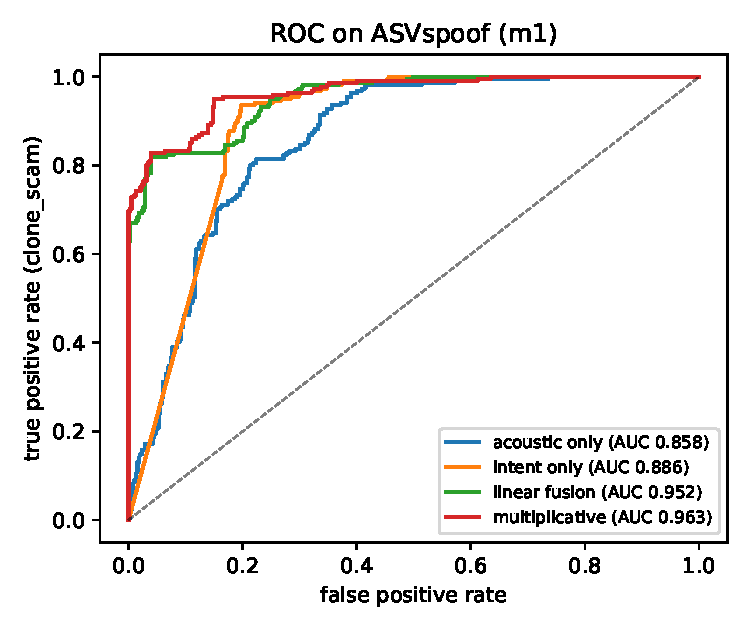
\includegraphics[width=0.6\linewidth]{F1_roc}
\caption{ROC on ASVspoof (m1). The multiplicative rule dominates.}
\label{fig:roc}
\end{figure}

\subsection{Multiplicative beats linear fusion}\label{sec:c2}
bayesian $-$ parallel, TPR@10\%FAR vs \textsc{genuine\_scam}, 8 seeds:
\begin{center}\small
\begin{tabular}{llcc}
\toprule
setting & acoustic regime & bayesian $-$ parallel & seeds won \\
\midrule
m1 $\times$ ASVspoof & informative, imperfect & $+0.251$ & 8/8 \\
m2 $\times$ In-the-Wild & informative, imperfect & $+0.136$ & 8/8 \\
m2 $\times$ ASVspoof & near-perfect (acoustic 0.994) & $-0.021$ & tie \\
m1 $\times$ In-the-Wild & broken (AUC 0.519) & $+0.001$ & n/a \\
\bottomrule
\end{tabular}
\end{center}
The multiplicative veto wins decisively in the informative-but-imperfect regime and is a
wash when the detector is near-perfect (nothing to fix) or broken (nothing to use). On
m1$\times$ASVspoof the bootstrap CI for bayesian on \textsc{genuine\_scam} $[0.674,0.858]$
does not overlap parallel's $[0.451,0.652]$. A third detector (mo-thecreator) exposes a
boundary: near-perfect on clean ASVspoof (tie), it collapses both classes to
P(synthetic)\,$\approx$\,0 under additive noise rather than degrading gracefully, leaving no
graded signal---so its gain is negative at every SNR. The veto's benefit is thus conditional
on the detector \emph{retaining a graded informative signal} in the imperfect regime (true
for m1, m2; false for m3), not merely on being ``imperfect.''

\subsection{Generalization is the binding constraint}\label{sec:c3}
Mean P(synthetic) by class:
\begin{center}\small
\begin{tabular}{lcc}
\toprule
model & ASVspoof genuine $\to$ clone & In-the-Wild genuine $\to$ clone \\
\midrule
m1 & $0.026 \to 0.401$ & $0.339 \to 0.211$ (inverted; AUC 0.519) \\
m2 & $0.353 \to 0.896$ & $0.212 \to 0.634$ \\
\bottomrule
\end{tabular}
\end{center}
The weaker detector collapses to chance on real-world deepfakes; the stronger SSL detector
transfers. When acoustic is broken, every method scores $\sim$0 against
\textsc{genuine\_scam}.

\subsection{Fusion gain vs.\ detector quality}\label{sec:sweep}
We add white noise at decreasing SNR (clean $\to$ 0\,dB), sweeping detector m2 from
informative to chance, and measure the multiplicative$-$linear gain against detector quality
(acoustic-only AUC). The gain is largest in the informative-but-imperfect band (AUC
$\approx0.73$--$0.86$), peaking at $+0.171$ on ASVspoof, and collapses to a tie when the
detector is near-perfect or at chance (Figure~\ref{fig:sweep}). On ASVspoof a small negative
dip appears in the weak-but-not-chance band, where absolute detection is low for both rules.

\begin{figure}[t]\centering
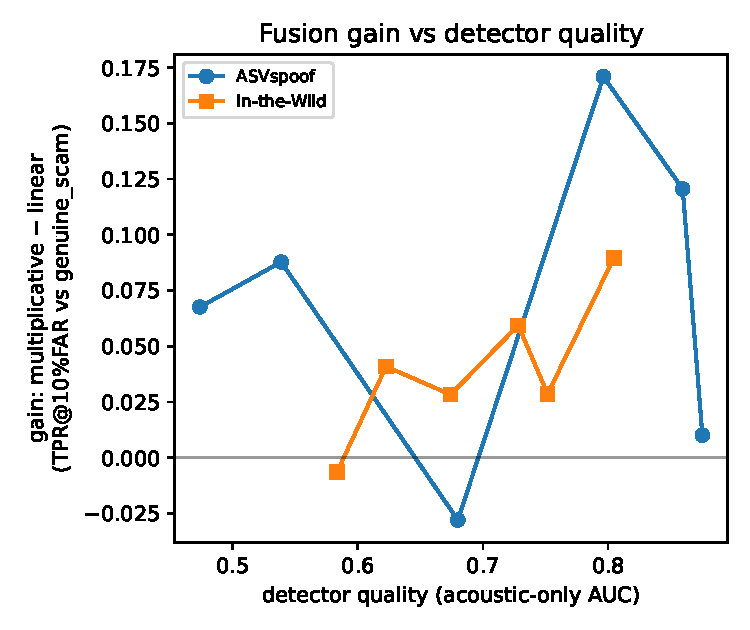
\includegraphics[width=0.6\linewidth]{F2_gain_vs_quality}
\caption{Multiplicative$-$linear fusion gain vs.\ detector quality; it peaks where the
detector is uncertain but not useless.}
\label{fig:sweep}
\end{figure}

\section{Limitations and ethics}
The benchmark pairs independent audio and transcripts, removing natural acoustic--content
correlation; real paired scam recordings would strengthen the evidence. The intent signal
is LLM-generated and LLM-scored, hence somewhat idealized. We evaluate three detectors, two
datasets, and one language, at modest scale (multi-seed reporting), and one degradation type
(additive noise); the veto's benefit is conditional on graceful detector degradation, which
not all detectors exhibit (\S\ref{sec:c2}). We study defense only,
introduce no new cloning capability, use public consented datasets, and release the
methodology to help defenders and establish prior art.

\section{Conclusion}
Fusing intent with an acoustic deepfake detector helps---conditionally. A multiplicative
acoustic veto is the right form precisely when the detector is informative but imperfect,
the regime real systems operate in. The dominant lever is acoustic-detector generalization:
when it fails, no fusion recovers it.

\appendix
\section{The simulation non-result}\label{sec:appendix}
A simulation favored a controller accumulating acoustic evidence over the call. We document
that this temporal advantage is a simulation artifact: real per-clip acoustic scores are
$\sim$constant across a call, so per-call scoring is appropriate and no streaming claim is
made.

\bibliographystyle{plain}
\bibliography{references}
\end{document}
